\documentclass[10pt]{article}
\usepackage{NotesTeX} %/Path/to/package should be replaced with package location
\usepackage{lipsum}
\usepackage{fontspec,fontenc,xunicode,xltxtra}
\usepackage{xeCJK}
\usepackage{tcolorbox}
\usepackage{caption}
\usepackage{graphicx, subfig}
\usepackage{multicol}
\setCJKmainfont[BoldFont = SimHei, ItalicFont = NSimSun]{宋体}
%\newtheorem{theorem}[definition]{corollary}[section]
\newtheorem{corollary}{Corollary}[section]
\tcolorboxenvironment{corollary}{
	boxrule=0pt,
	boxsep=0pt,
	blanker,
	borderline west={2pt}{0pt}{Green},
	before skip=10pt,
	after skip=10pt,
	left=12pt,
	right=12pt,
	breakable,
}

\title{{\Huge 数值计算实验上机报告6.2}\\}
\author{吴尊和}

\emailAdd{wuzunhe@gmail.com}
\begin{document}
  \maketitle
  \flushbottom
  \newpage
  \pagestyle{fancynotes}
  \part{题目}
  通过上机计算,分析了古典迭代法中的GS,J方法的迭代步数差距;讨论了SOR方法的松弛因子对迭代步数的影响,并找到相应的最佳迭代银子,并比较了上述三种迭代法。而后通过对变系数R方法与半迭代加速J方法的观察,了解了算法中的重启技术,并且讨论了重启技术中循环指标$m$的影响;了解了CG算法以及用SSOR作为预处理因子的PCG算法,考察了这两个算法与之前的SOR算法的异同。
  
  \newpage
  \pagestyle{fancynotes}
  \part{数学原理}
  \section{基本理论}
  \indent 所谓迭代解法就是通过简单的计算规则,自动生成一个向量序列
  \begin{equation}x_k=f_k(x_{k-1},x_{k-2},\cdots,x_{k-r}),\indent k\leq r,
  \end{equation}
  其中前$r$个向量${x_k}_{k=0}^{r-1}$是需要人工给出的启动初值。由于迭代函数$f_k$包含$r$个历史信息,故而称该方法是$r$阶的。若迭代函数同迭代步数$k$无关,则称方法是定常的;否则,称方法是非定常的。
  \subsection{一阶迭代方法}
  为简单起见,首先讨论线性方程组$\mathbb{A}x=b$的一阶迭代方法。通常,它具有两种表现形式:
  \begin{align}
  &x_k=x_{k-1}+\mathbb{H}_k(b-\mathbb{A}x_{k-1})=x_{k-1}-\mathbb{H}_kr_{k-1},\\
  &x_k=\mathbb{G}_kx_{k-1}+g_k,
  \end{align}
  其中$\mathbb{H}_k$称为预处理矩阵,$\mathbb{G}_k$称为迭代矩阵,
  $$r_k=\mathbb{A}x_k-b$$称为残量。若$r_k=0$,则$x_k=x_*$是精确解。\newline
  因此,迭代方法的研究重点是如何构造迭代矩阵(或者预处理矩阵),使$x_k$能够快速地收敛到精确解。
  \subsection{收敛速度的刻画与估计}
  通常用误差向量$e_k$趋于零的(最坏)速度,衡量迭代算法的收敛快慢。譬如,一阶定常迭代方法$x_k=\mathbb{G}x_{k-1}+g$满足误差估计
  \begin{equation}
  \Vert e_k\Vert\leq\Vert\mathbb{G}^k\Vert\Vert e_0\Vert.
  \end{equation}
  右端系数$\Vert\mathbb{G	}^k\Vert$通常是无法改善的,因为等号成立的情形是真实存在的。下面以这个极端保守的数量$\Vert\mathbb{G}^k\Vert$,作为收敛速度的讨论起点。
  \begin{definition}[收敛速度]
  为直观起见,通常用误差下降的平均效应刻画迭代误差趋于零的速度:
  \begin{enumerate}
  \item 平均收敛速度\indent $R_k(\mathbb{G})=-\frac{1}{k}ln\Vert\mathbb{G}^k\Vert$;
  \item 渐进收敛速度\indent $R_{\infty}(\mathbb{G})=\lim_{k\rightarrow\infty}R_k(\mathbb{G})=-ln\rho(\mathbb{G}).$
  \end{enumerate}
  \end{definition}
  \begin{theorem}
  若$\mathbb{G}<1$,则定常迭代方法$x_k=\mathbb{G}x_{k-1}+g$是收敛的。相应的迭代误差满足\begin{enumerate}
  \item 先验误差估计:\indent $\Vert e_k\Vert\leq\Vert\mathbb{G}\Vert^k\Vert e_0\Vert;$
  \item 后验误差估计$(\uppercase\expandafter{\romannumeral1})$:\indent$\Vert e_k\Vert\leq\frac{\Vert\mathbb{G}\Vert}{1-\Vert\mathbb{G}\Vert}\Vert x_k-x_{k-1}\Vert;$
  \item 后验误差估计$(\uppercase\expandafter{\romannumeral2})$:\indent$\Vert e_k\Vert\leq\frac{\mathbb{G}^k}{1-\Vert\mathbb{G}\Vert}\Vert x_1-x_0\Vert,$
  \end{enumerate}
  其中$\delta_k\equiv\Vert x_k-x_{k-1}\Vert $称为相邻误差,也是可以直接计算的。
  \end{theorem}
  \subsection{停机标准}
  在迭代方法中,何时停机也是一个重要的问题。当然,我们希望数值误差达到用户要求 
  \begin{equation}
  \Vert e_k\Vert\leq \epsilon
\end{equation}    
即可停机,其中$\epsilon$是用户事先给出的停机指标。但是,这种停机策略只能作于理论研究(或数值实验),因为迭代误差是无法计算的量。\newline
实际计算常常采用下面三个停机准则,特别是后两个同准则(1.5)没有明确的等价关系。它们分别是:
\begin{enumerate}
\item 残量准则:$\Vert r_k\Vert\leq\epsilon;$
\item 相邻误差准则:$\delta_k\leq\epsilon;$
\item 后验误差停机准则:$\delta_k^2/(\delta_{k-1}-\delta_k)\leq\epsilon.$
\end{enumerate}
\section{古典迭代算法}
	$J$方法基于同步更新策略,而$GS$方法基于异步更新策略。迭代序列按照如下方式更新每个分量:
	\begin{enumerate}
	\item $J$方法:\indent $x_k^{(i)}=\frac{1}{a_{ii}}[b^{(i)}-\sum_{j\neq i}a_{ij}x_{k-1}^{(j)}],$
	\item $GS$方法:\indent $x_k^{(i)}=\frac{1}{a_{ii}}[b^{(i)}-\sum_{j< i}a_{ij}x_{k}^{(j)}-\sum_{j>i}a_{ij}x_{k-1}^{(j)}].$
	\end{enumerate}
\section{逐次超松弛方法}
逐次超松弛方法具有极其重要爱的历史地位,它极大地拓展了迭代方法的设计思路:对旧的迭代序列进行加权平均,可以期待新的迭代序列具有更快的收敛速度。
\begin{definition}
	$SOR$方法是以$GS$方法为蓝本,逐一加权平均两个新旧向量的对应分量。具体更新方式是
	$$x_k^{(i)}=(1-\omega)x_{k-1}^{(i)}+\frac{\omega}{a_{ii}}[b^{(i)}-\sum_{j<i}a_{ij}x_k^{(j)}-\sum_{j>i}a_{ij}x_{k-1}^{(j)}],$$其中$\omega$称为松弛因子,相应的迭代矩阵是
	\begin{equation}
	\mathbb{T}_{\omega}=(\mathbb{I}-\omega\mathbb{L})^{-1}[(1-\omega)\mathbb{I}+\omega\mathbb{U}].
	\end{equation}
	显然,当$\omega=1$,$SOR$方法就是$GS$方法。
\end{definition}
\subsection{收敛性}
为保证$SOR$方法收敛,松弛因子$\omega$要满足适当条件。
\begin{theorem}
$SOR$方法收敛的必要条件是$0<\omega<2.$
\end{theorem}
\begin{theorem}
若系数矩阵$\mathbb{A}$对称正定,则$0<\omega<2$是$SOR$方法收敛的充分必要条件。
\end{theorem}
\section{迭代加速方法}
$SOR$方法的研究结果表明:充分利用已有的计算信息,可以有效提高收敛速度。为此,本节介绍基础迭代方法
\begin{equation}
x_k=\mathbb{G}x_{k-1}+g
\end{equation}的两种常用迭代加速技术,特别是著名的半迭代方法。
\subsection{外推方法}
\begin{definition}
外推方法是$SOR$方法的直接推广。设$\gamma$是给定的权重,加权平均相邻的两个数值解,定义
$$x_k=\gamma(\mathbb{G}x_{k-1}+g)+(1-\gamma)x_{k-1}.$$
\end{definition}
\subsection{半迭代方法}
半迭代方法可以看作外推思想的极致推广。换言之,我们想充分利用已知的所有计算结果,通过适当的加权平均处理,期待
\begin{equation}
y_m=\sum_{k=0}^m \alpha_{m,k}x_k
\end{equation}
比$x_k$更加接近精确解,其中$\lbrace x_k\rbrace_{k=0}^{\infty}$是由基础迭代算法(4.1)给出的迭代序列。
若$x_k\equiv x_{*}$是精确解,则$y_m\equiv x_{*}$应当也是精确解。因此,参数组$\lbrace \alpha_{m,k}\rbrace_{k=0}^{m}$应满足相容性条件
\begin{equation}
\sum_{k=0}^{m}\alpha_{m,k}=1.
\end{equation}
记$\eta_m=y_m-x_{*}$是半迭代法(4.2)的第$m$步误差。简单计算可知,其误差方程为
\begin{equation}
\eta_m=\sum_{k=0}^{m}\alpha_{m,k}\mathbb{G}^{k}e_0=\mathbb{P}_m(\mathbb{G})e_0,
\end{equation}
其中$e_0=\eta_0=x_0-x_{*}$为初始误差。这里的$\mathbb{P}_m(\lambda)s$是$m$次多项式,相应的系数由参数组$\lbrace\alpha_{m,k}\rbrace_{k=0}^m$给出。至此,一种新的构造思想诞生了,迭代方法的研究思路也从“单项式算法”拓展到“多项式算法”。\newline
基于误差方程(4.4),自然希望$\mathbb{P}_m(\mathbb{G})$的谱半径远远小于$\mathbb{G}$的谱半径。为此,研究中心是寻找$\mathbb{P}_m(\mathbb{G})$的谱半径的最小值,给出线性组合的最佳权重。
\subsubsection{变系数Richardson方法}
事实上,某些传统算法已经隐含地实现了半迭代法的基本思想,一个典型实例是$Richardson$迭代方法
\begin{equation}
x_k=x_{k-1}+\tau_k(b-\mathbb{A}x_{k-1}),
\end{equation}其中$\tau_k$是可以变化的迭代参数。显而易见,$R$方法可以理解为残量松弛方法,比$J$方法更加简单。其中有
\begin{equation}
\tau_k^{*}=\frac{\lambda_{max}-\lambda_{min}}{2}cos(\frac{2k-1}{2m}\pi)+\frac{\lambda_{max}+\lambda_{min}}{2}.
\end{equation}为最佳参数组。
\subsubsection{Cheybeshev加速方法}
再次考虑半迭代方法(4.2),讨论最佳参数组$\lbrace\alpha_{m,k}\rbrace_{k=0}^m$的设置及效果;同时,半迭代方法还需给出相应的实现途径,解决数据存储的困境。 设基础迭代方法(4.1)的迭代矩阵$\mathbb{G}$是实对称的,此时$\mathbb{G}$具有完备的特征向量系$\lbrace \xi_i\rbrace_{k=1}^{n},$相应的特征值$\lbrace \lambda_i\rbrace_{i=1}^{n}$均为实数。初始误差可以表达为$$e_0=\sum_{1\leq i\leq n}\beta_i\xi_i,$$其中$\beta_i$是已知常数。由误差方程(4.4)可知,半迭代方法(4.2)的迭代误差满足$$e_k=\sum_{i=1}^n[\sum_{l=0}^{k}\alpha_{k,l}\lambda_i^{l}]\beta_i\xi_i=\sum_{i=1}^{n}Q_k(\lambda_i)\beta_i\xi_i.$$,有一组最佳参数$\lbrace\alpha_{m,k}\rbrace_{k=0}^m$,使得迭代误差趋于零的速度达到最快。事实上,考虑最佳多项式\begin{equation*}
Q_k^{*}(\lambda)=\frac{T_k(l(\lambda))}{T_k(l(1))},
\end{equation*}
其中$T_k(z)$为标准的$Chebyshev$多项式,
\begin{equation}
l(\lambda)=\frac{2\lambda-\lambda_{max}-\lambda{min}}{\lambda{max}-\lambda{min}}.
\end{equation}
,而最佳参数组就是$Q_k^*(\lambda)$的相应系数。
\subsection{共轭斜量法}
共轭斜量($CG=Conjurate Gradient$)法是对称正定线性方程组的首选数值方法。其核心思想是利用合适的优化方法,快速求解等价的目标函数极值点。它无需事先估计系数矩阵的特征值,具有无参数和快速收敛等优势。
\subsubsection{共轭斜量系的构造过程}
彼此垂直的$r_{k+1}$和$p_k$局部张成一个二维平面,它包含一个$\mathbb{A}$-共轭于$p_k$的搜索方向$p_{k+1}$。基于这个思路,定义算法如下:
\newline 令$p_0=-r_0=b-\mathbb{A}x_0,$依次执行
\begin{enumerate}[]
	\item $x_{k+1}=x_k+\alpha_k p_k,\indent \alpha_k=-\frac{r_k^Tp_k}{p_k^T\mathbb{A}p_k},$
	\item $r_{k+1}=r_k+\alpha_k\mathbb{A}p_k,$
	\item $p_{k+1}=-r_{k+1}+\beta_k p_k,\indent\beta_k=\frac{r_{k+1}^T\mathbb{A}p_k}{p_k^T\mathbb{A}p_k}.$
\end{enumerate}
\subsubsection{预处理共轭斜量方法}
预处理技术是数值代数的基本技术。它用于改善线性方程组的条件数(或者特征值的分布属性),从而提高算法的计算效率。\newline
下面以共轭斜量方法为例,阐述预处理技术的基本思想和实现过程。设预处理矩阵是$\mathbb{Q} = \mathbb{C}\mathbb{C}^T$,考虑同解方程组$$\mathbb{C}^{-1}\mathbb{A}\mathbb{C}^{-T}\mathbb{C}^{T}x=\mathbb{C}^{-1}b$$的CG算法,则计算流程如下\newline
令$r_0=\mathbb{A}x_0-b$,令$z_0=\mathbb{Q}^{-1}r_0,p_0=-z_0$依次执行
\begin{enumerate}[]
	\item $x_{k+1}=x_k+\alpha_k p_k,\indent \alpha_k=-\frac{r_k^Tz_k}{p_k^T\mathbb{A}p_k},$
	\item $r_{k+1}=r_k+\alpha_k\mathbb{A}p_k,$
	\item $z_{k+1}=\mathbb{Q}^{-1}r_{k+1},$
	\item $p_{k+1}=-z_{k+1}+\beta_k p_k,\indent\beta_k=\frac{r_{k+1}^Tz_{k+1}}{r_k^Tz_k}.$
\end{enumerate}
  \newpage
  \pagestyle{fancynotes}
  \part{实验结果}
  \begin{enumerate}
  \item 分别采用残量、相邻差量和后验误差作为停机标准, 比较 J 方法和 GS 方法停机时的迭代次数和真实误差。
  \begin{figure}[H]
  \centering
  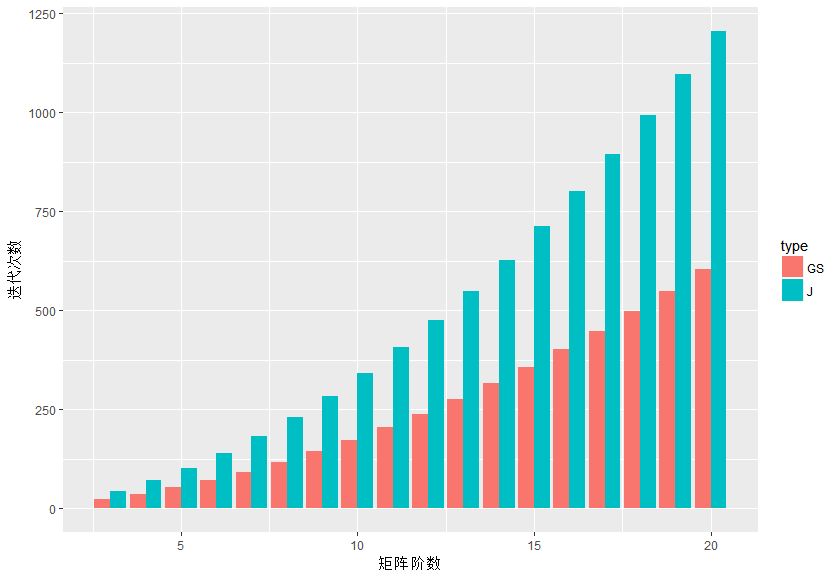
\includegraphics[width=.9\textwidth]{1-1.png}
  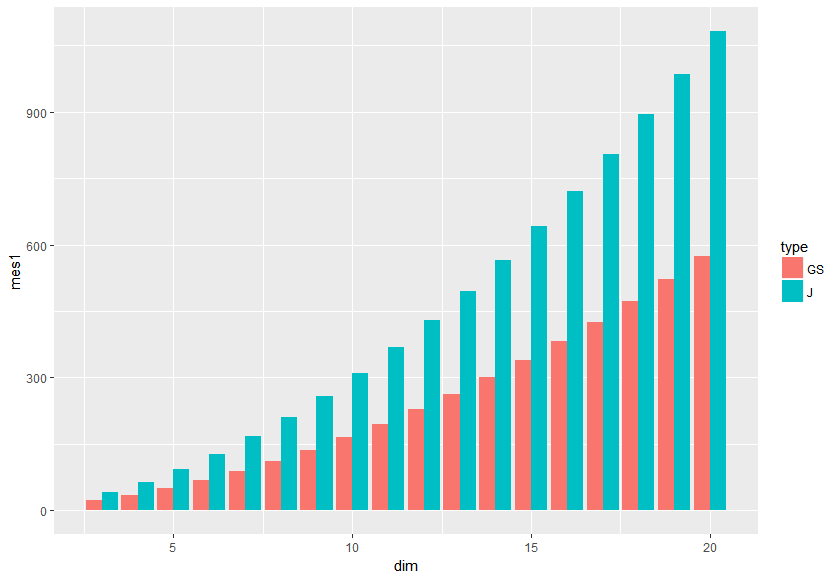
\includegraphics[width=.9\textwidth]{1-2.png}
  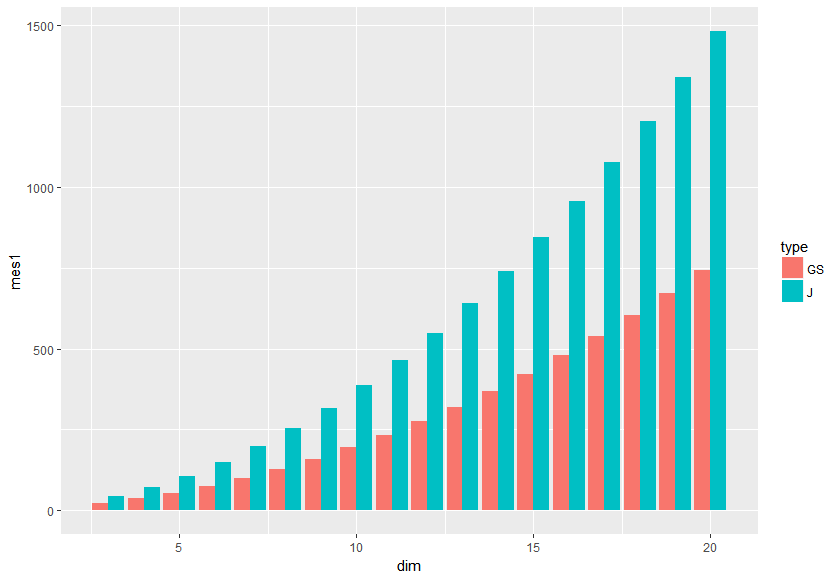
\includegraphics[width=.9\textwidth]{1-3.png}
  \caption{J于GS的对比}
  \end{figure}
  显然,$J$方法的迭代速度为$GS$的方法的两步。迭代次数随结束增大而增大。同时,当停机后,$GS$得出的解也同样更接近于真解。
  \begin{figure}[H]
  \centering
  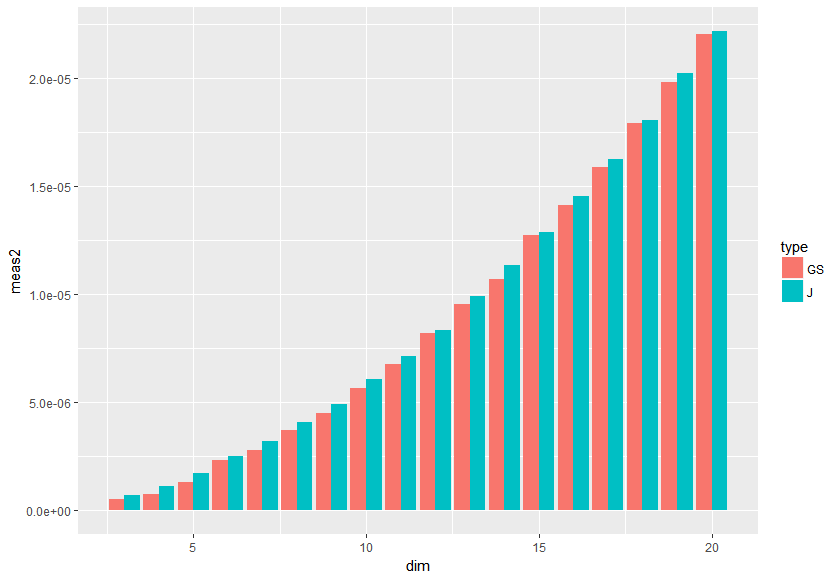
\includegraphics[width=.9\textwidth]{1111.png}
  \caption{J于GS的对比}
  \end{figure}
  \item  以真实误差作为停机标准,数值观察$SOR$方法的松弛因子$\omega$对于迭代次数的影响,并找到相应的最佳迭代因子。
  \begin{figure}[H]
  \centering
  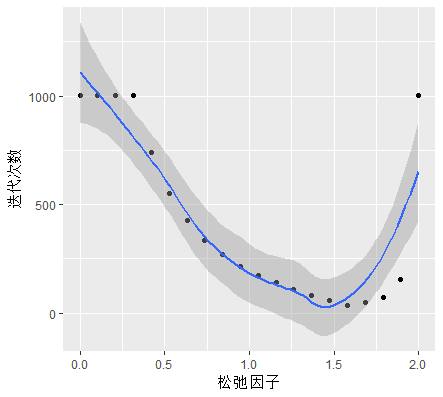
\includegraphics[width=.8\textwidth]{2.png}
  \end{figure}
  如图所示,当松弛因子$\omega$在$(1.47,1.68)$的范围内时由较好的迭代加速效果,此时只需迭代36次左右即可达到目标精度。\newline
  此外,由图可知松弛因子$\omega$在区间$(0,\omega_{opt})$内随着松弛因子的变大使得迭代次数下降,在$(\omega_{opt},2)$内随着松弛因子变大使得迭代次数上升。
  \item  考虑$J$方法、$GS$方法和(带有最佳松弛因子的)$SOR$方法,进行下面的数值观察:\begin{enumerate}
  \item 绘制相应的误差曲线和残量曲线,均采用半对数坐标系;
  \begin{figure}[H]
  \centering
  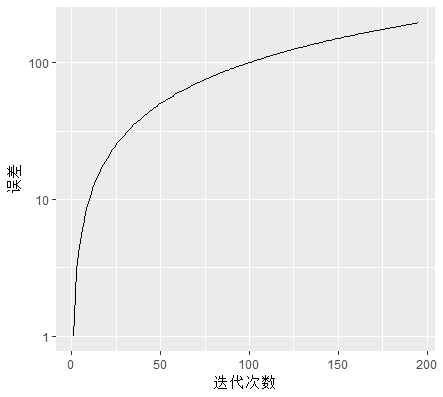
\includegraphics[width=.9\textwidth]{3-G1.png}
  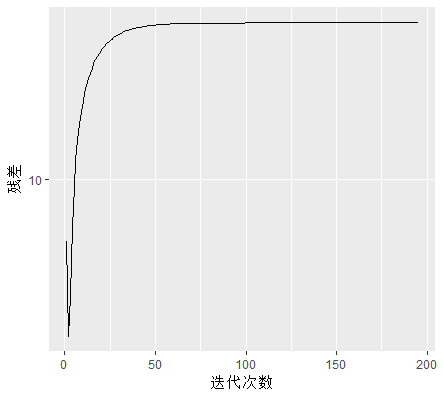
\includegraphics[width=.9\textwidth]{3-G2.png}
  \caption{GS}
  \end{figure}
  \begin{figure}[H]
  \centering
  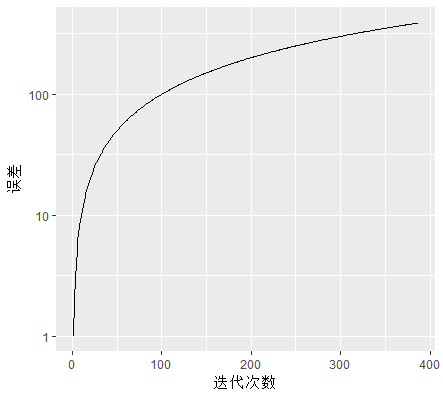
\includegraphics[width=.9\textwidth]{3-J1.png}
  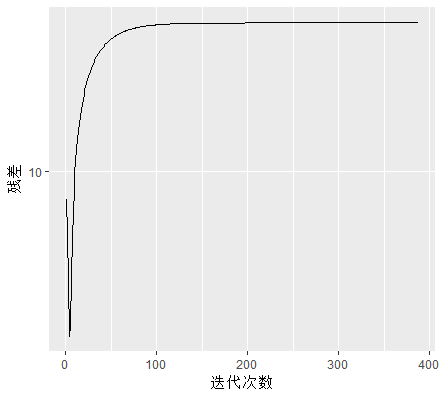
\includegraphics[width=.9\textwidth]{3-J2.png}
  \caption{J}
  \end{figure}
\begin{figure}[H]
  \centering
  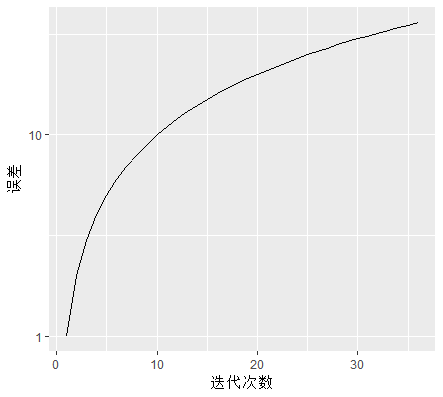
\includegraphics[width=.9\textwidth]{3-S1.png}
  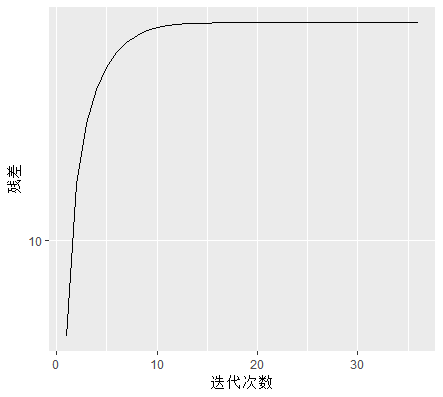
\includegraphics[width=.9\textwidth]{3-S2.png}
  \caption{Sor}
  \end{figure}	
	\item  以真实误差为停机标准,绘图指出迭代次数同矩阵阶数的关系。
	\begin{figure}[H]
  \centering
  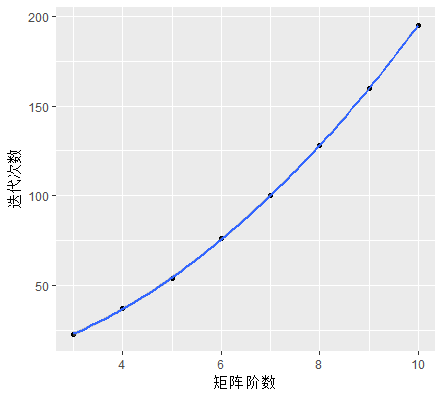
\includegraphics[width=.9\textwidth]{32-Gauss.png}
  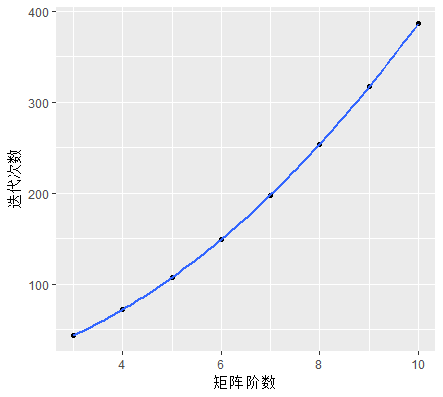
\includegraphics[width=.9\textwidth]{32-Jacobi.png}
  \includegraphics[width=.9\textwidth]{32-Sor.png}
  \caption{迭代次数同矩阵阶数的关系}
  \end{figure}
  \end{enumerate}
\item 绘制变系数R方法的误差曲线以及残量曲线,观测循环指标m的影响。
\begin{figure}[H]
  \centering
  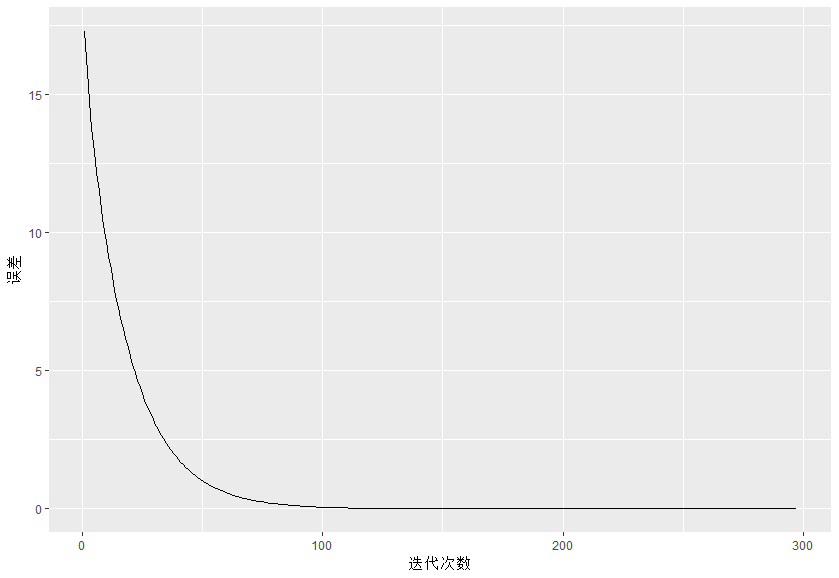
\includegraphics[width=.8\textwidth]{4-m=51.png}
  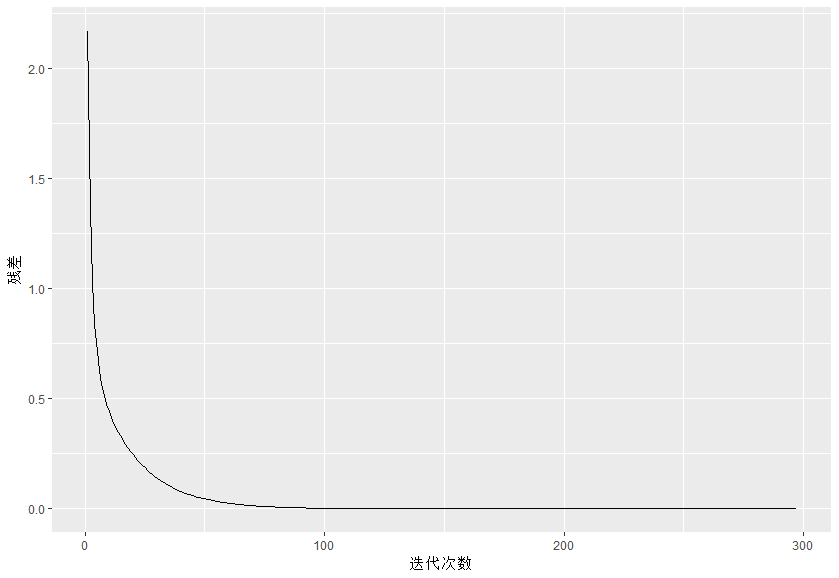
\includegraphics[width=.8\textwidth]{4-m=52.png}
  \caption{m=5}
  \end{figure}
  \begin{figure}[H]
  \centering
  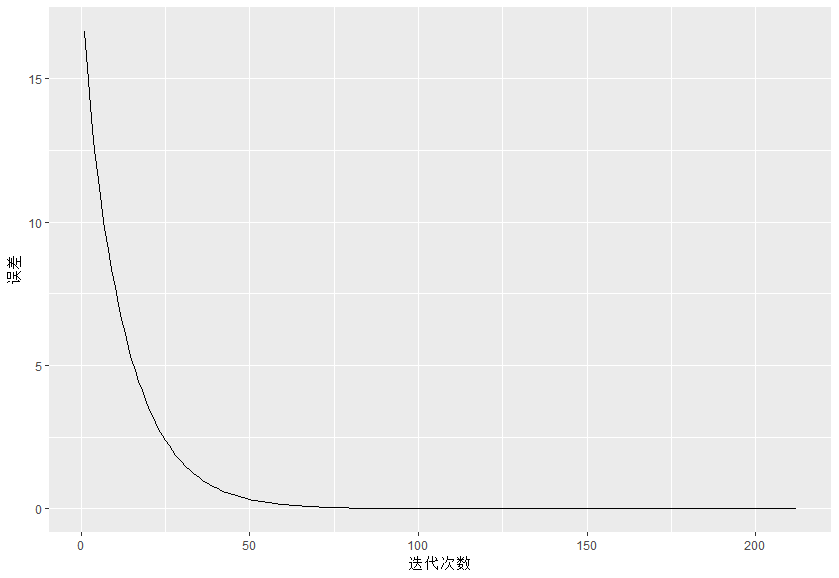
\includegraphics[width=.8\textwidth]{4-m=71.png}
  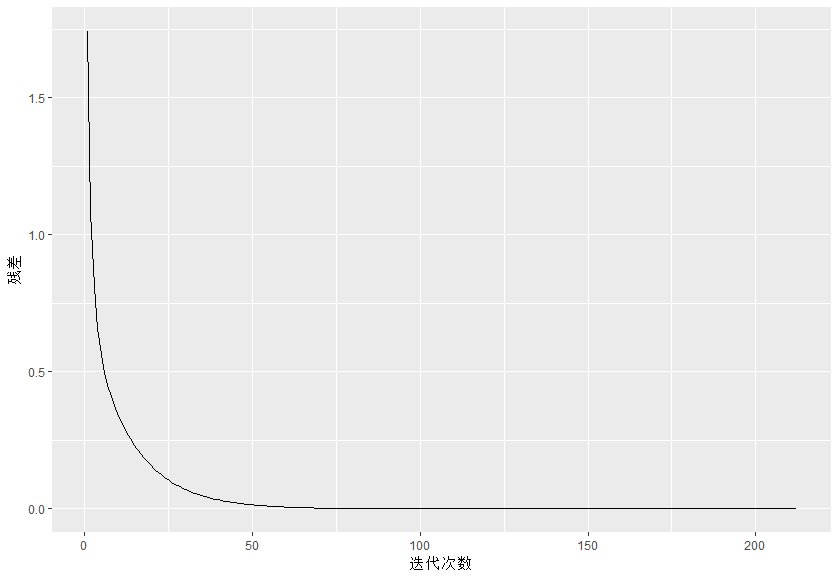
\includegraphics[width=.8\textwidth]{4-m=72.png}
  \caption{m=7}
  \end{figure}
  \begin{figure}[H]
  \centering
  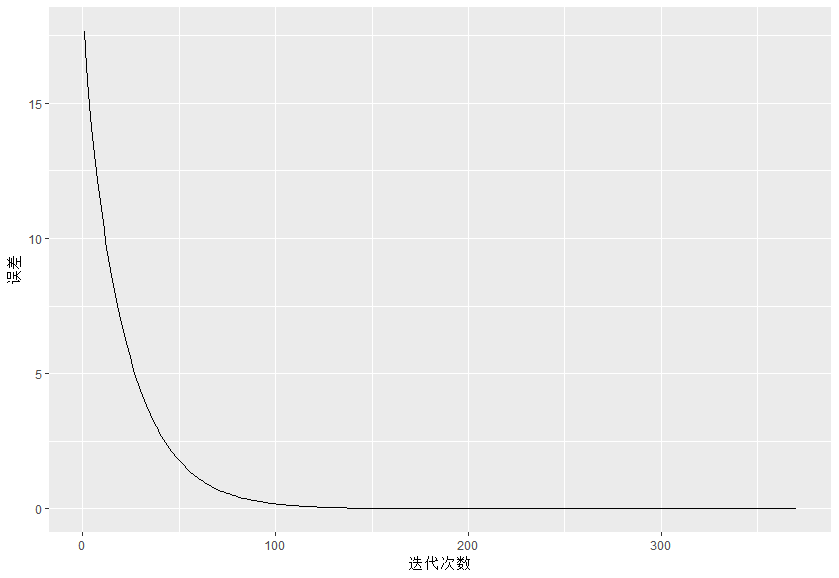
\includegraphics[width=.8\textwidth]{4-m=81.png}
  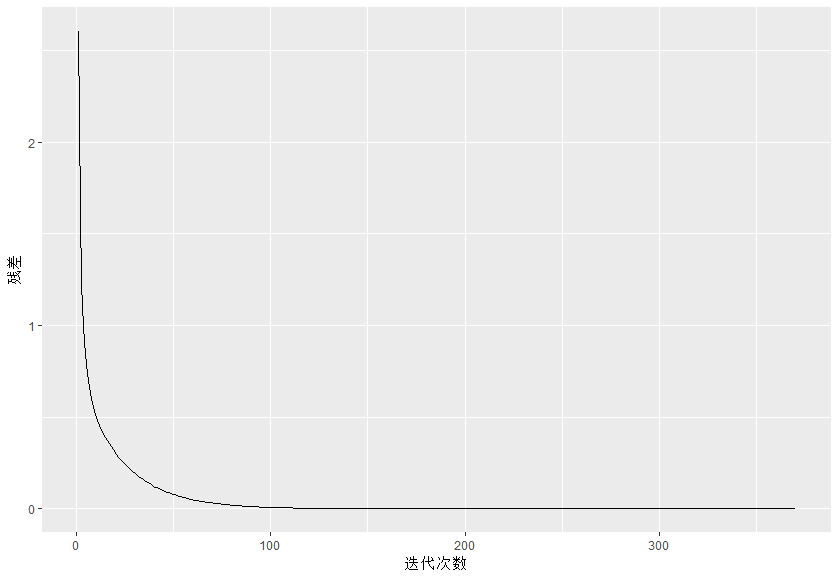
\includegraphics[width=.8\textwidth]{4-m=82.png}
  \caption{m=8}
  \end{figure}
  \begin{figure}[H]
  \centering
  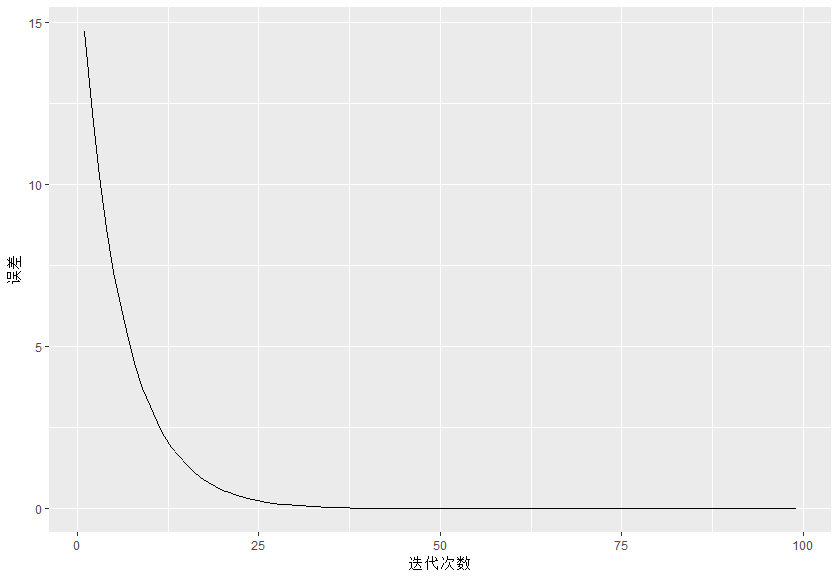
\includegraphics[width=.8\textwidth]{4-m=151.png}
  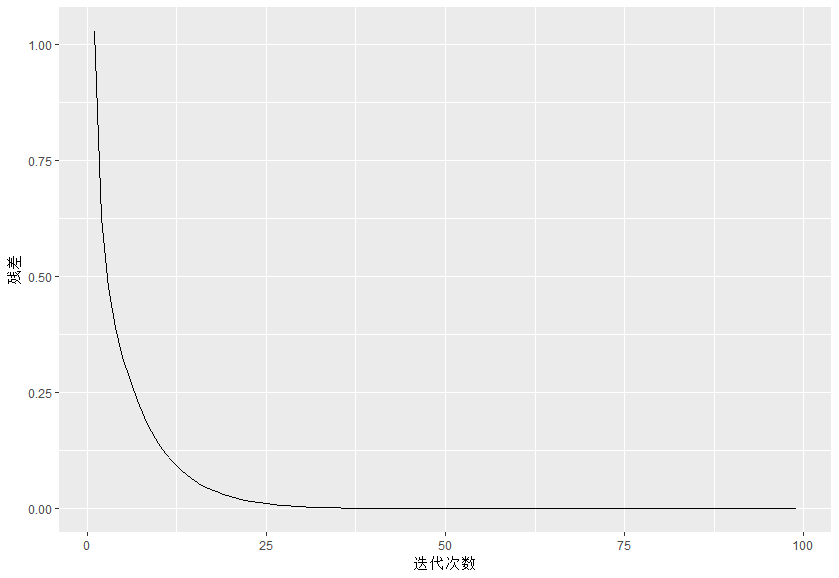
\includegraphics[width=.8\textwidth]{4-m=152.png}
  \caption{m=15}
  \end{figure}
  \begin{figure}[H]
  \centering
  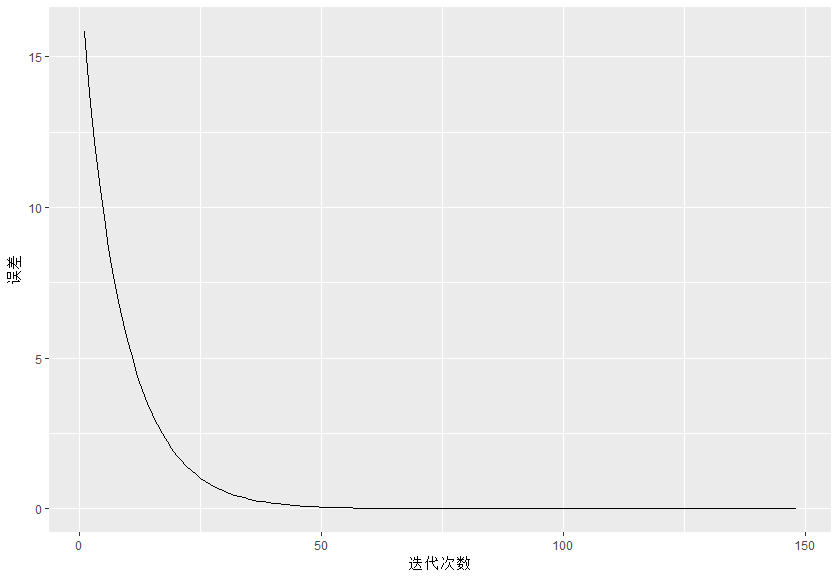
\includegraphics[width=.8\textwidth]{4-m=201.png}
  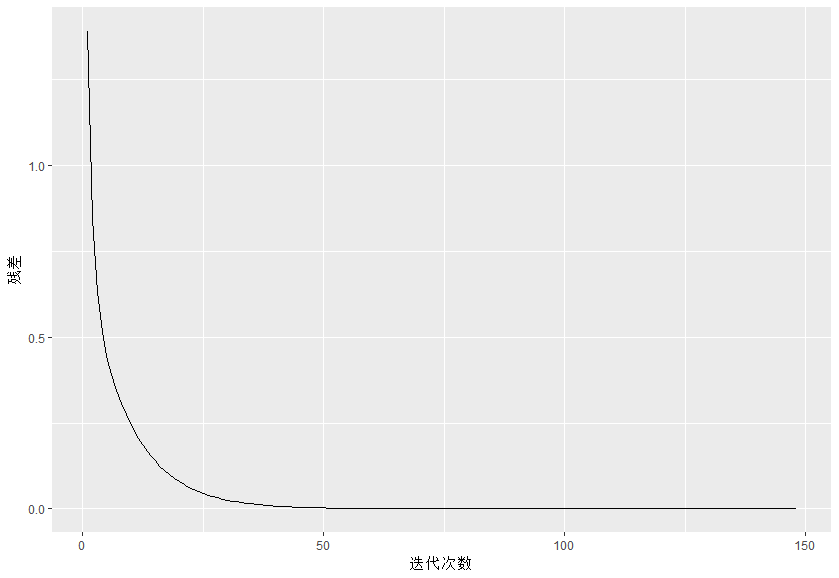
\includegraphics[width=.8\textwidth]{4-m=202.png}
  \caption{m=20}
  \end{figure}
  由图可知,指标$m$会影响迭代法收敛的速度,但该影响并非正相关也非负相关的。同时我们也从图像的形状中可以得出,在迭代法前期收敛趋向真解的速度较后期更快。
\item 取循环指标$m=5$,半迭代加速$J$方法;绘制相应的误差曲线和残量曲线,其他的$m$呢?
\begin{figure}[H]
  \centering
  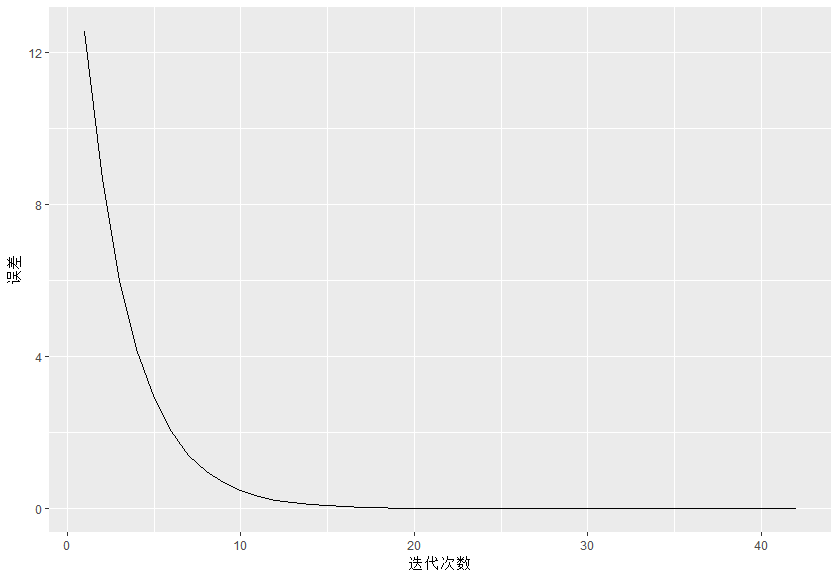
\includegraphics[width=.8\textwidth]{5-m=51.png}
  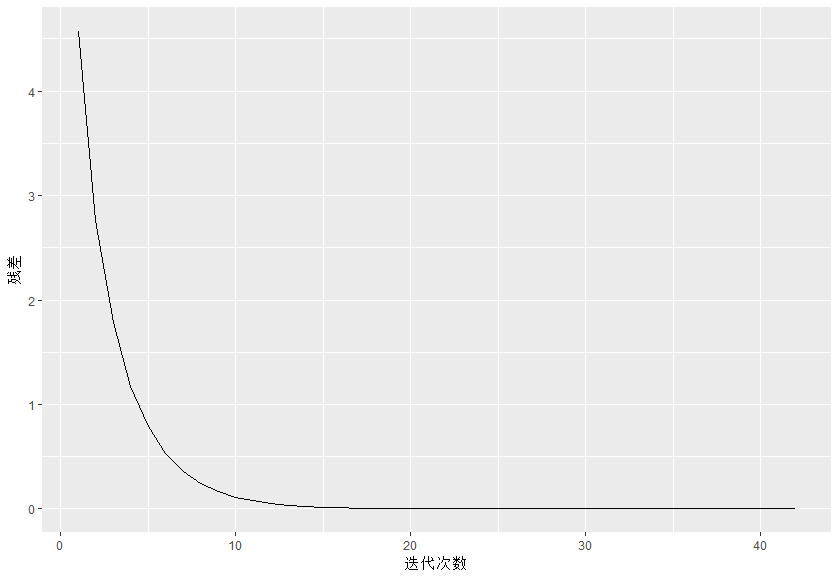
\includegraphics[width=.8\textwidth]{5-m=52.png}
  \caption{m=5}
  \end{figure}
  
\begin{figure}[H]
  \centering
  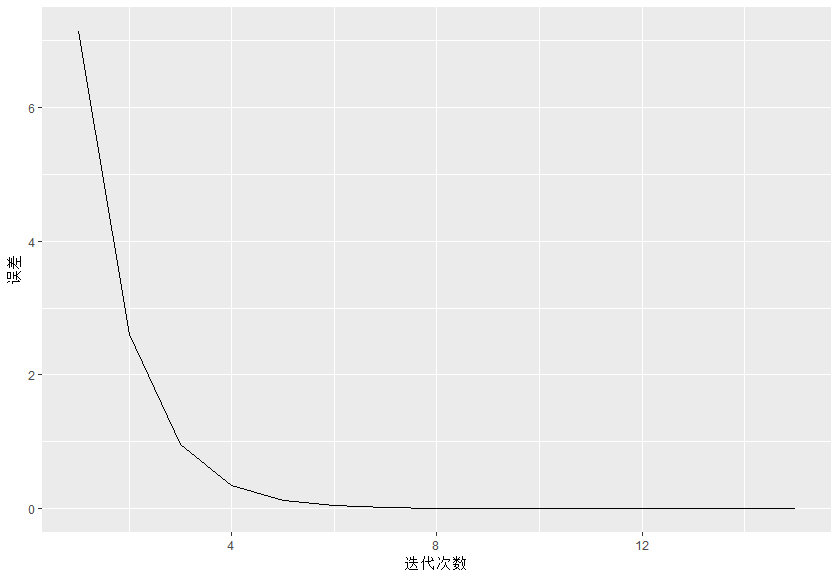
\includegraphics[width=.8\textwidth]{5-m=101.png}
  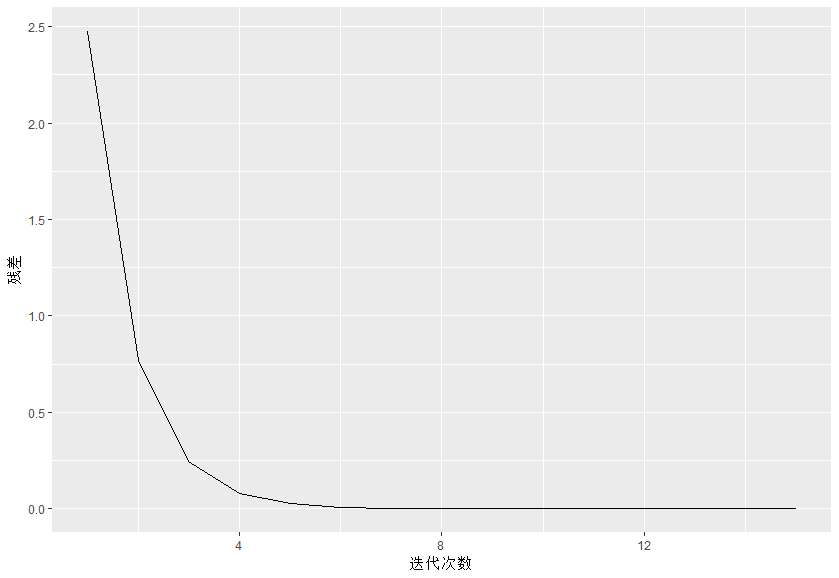
\includegraphics[width=.8\textwidth]{5-m=102.png}
  \caption{m=10}
  \end{figure}
  
\begin{figure}[H]
  \centering
  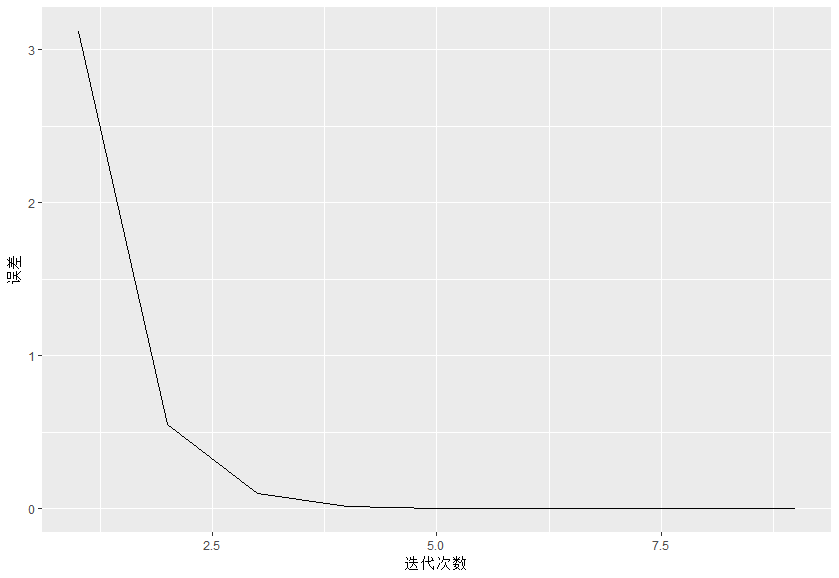
\includegraphics[width=.8\textwidth]{5-m=151.png}
  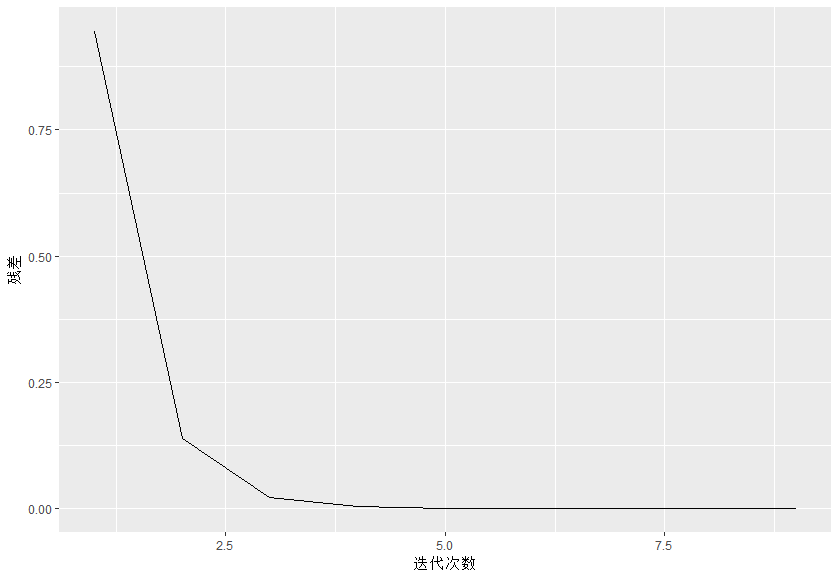
\includegraphics[width=.8\textwidth]{5-m=152.png}
  \caption{m=15}
  \end{figure}
  
\begin{figure}[H]
  \centering
  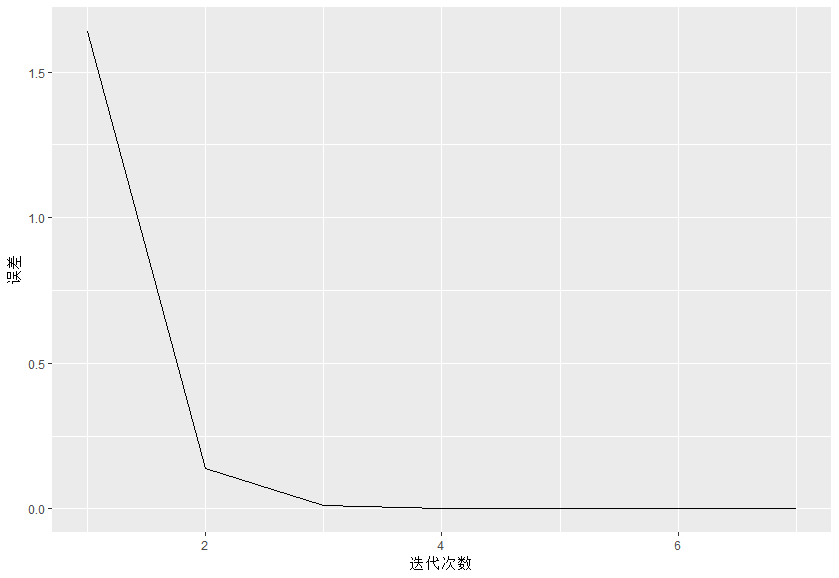
\includegraphics[width=.8\textwidth]{5-m=201.png}
  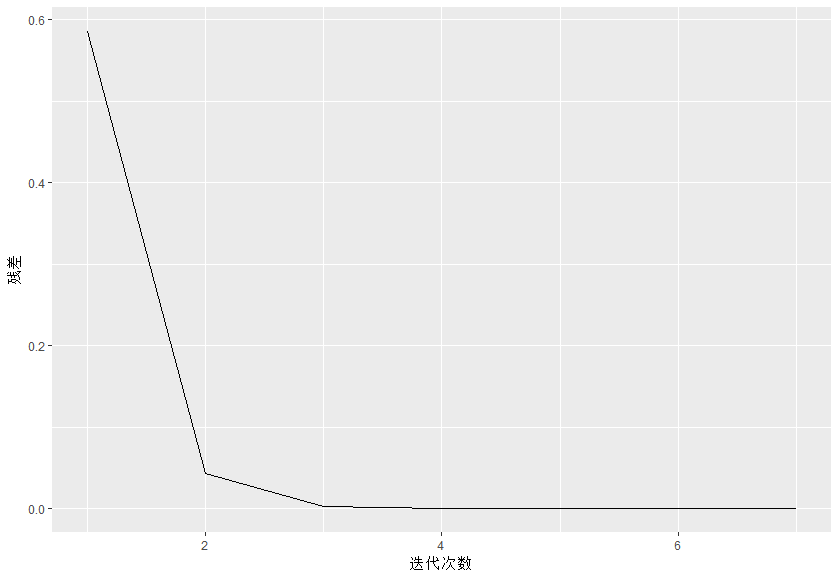
\includegraphics[width=.8\textwidth]{5-m=202.png}
  \caption{m=20}
  \end{figure}
  观察图像,我们可以得出在用半迭代法加速$Jacobi$方法时,$m$的值越大,迭代次数递减,故在不会导致较大的舍入误差的情况下m越大越好。
\item 执行CG方法,进行下面的数值观察:
\begin{enumerate}
\item 取$n=31$和$n=32$两种奇偶状态,绘制相应的误差曲线和残量曲线;

\begin{figure}[H]
  \centering
  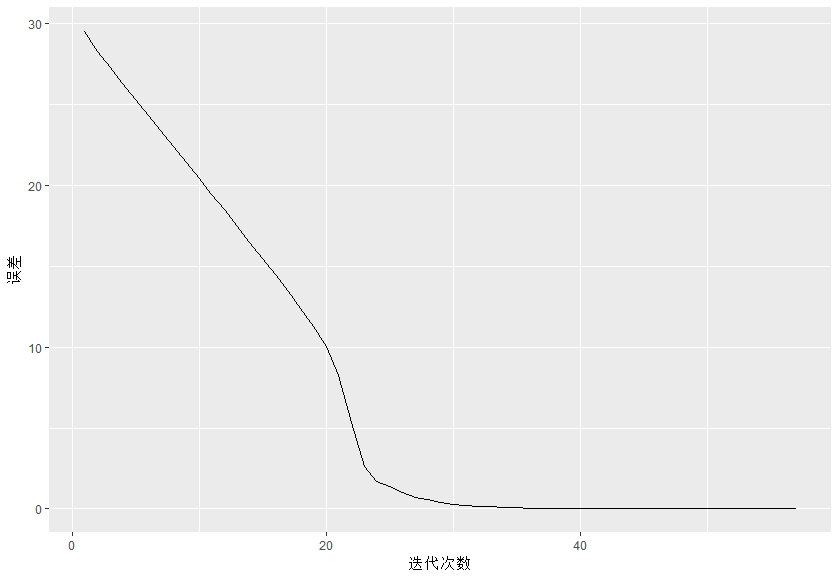
\includegraphics[width=.9\textwidth]{6-a-311.png}
  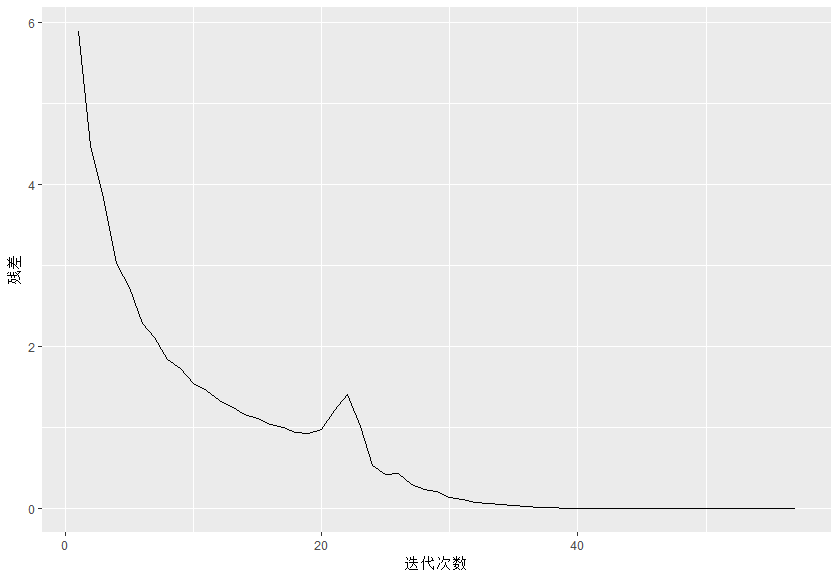
\includegraphics[width=.9\textwidth]{6-a-312.png}
  \caption{n=31}
  \end{figure}
 \begin{figure}[H]
  \centering
  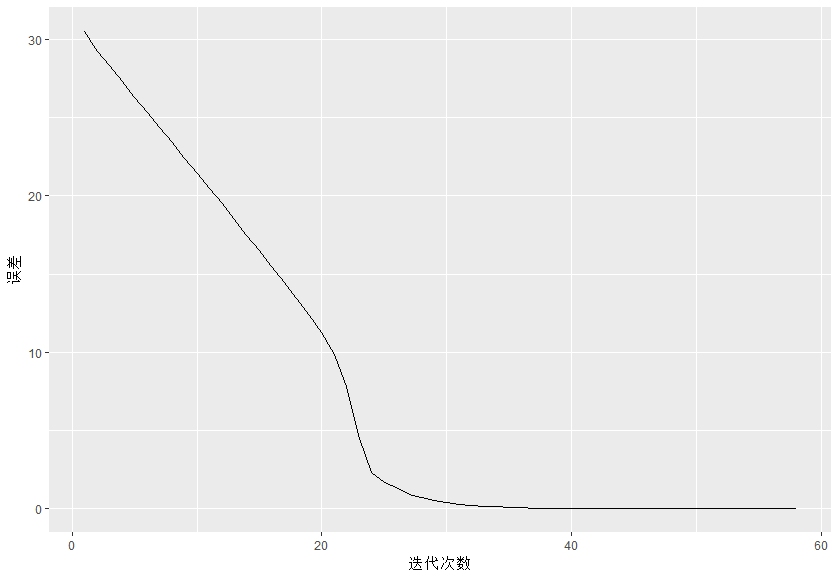
\includegraphics[width=.9\textwidth]{6-a-321.png}
  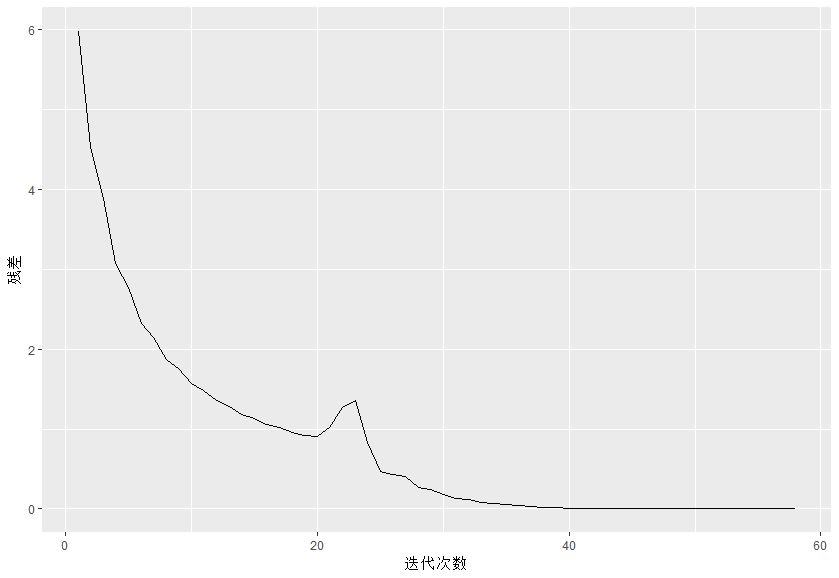
\includegraphics[width=.9\textwidth]{6-a-322.png}
  \caption{n=32}
  \end{figure}
\item 绘图指出迭代次数同矩阵阶数的关系,比较这个关系同SOR方法的差异。
\begin{figure}[H]
  \centering
  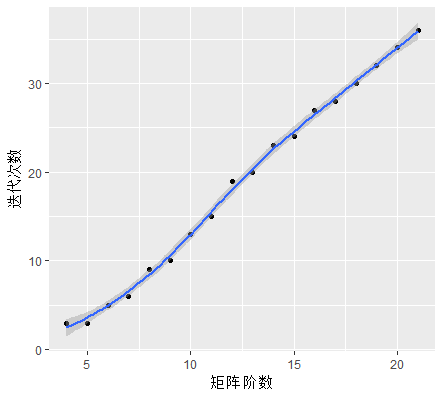
\includegraphics[width=.9\textwidth]{CGb.png}
  \end{figure}
\end{enumerate}
\item 采用SSOR做为预处理因子,编制相应的预处理CG算法。随机取定矩阵阶数,考察迭代次数同参数$\omega$的关系。
\begin{figure}[H]
  \centering
  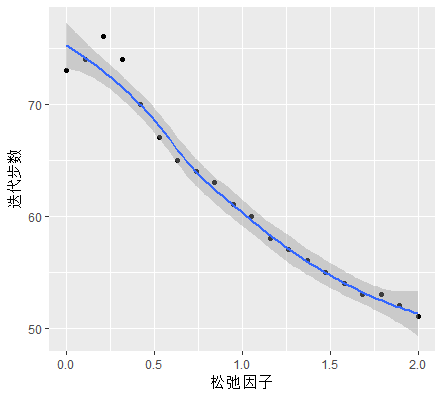
\includegraphics[width=.9\textwidth]{lastone.png}
  \caption{PCG}
  \end{figure}
  从图中信息可知,迭代步数随着$\omega$的增大而减少,似乎此时的$\omega$甚至可以超过2.
  \end{enumerate}
  \newpage
  \pagestyle{fancynotes}
  \part{小结}
  \begin{enumerate}
  \item $Jacobi$迭代的步数约等于$GS$方法的迭代步数的两倍,且相同停机准则的情况下,$GS$方法所得到的解更接近于真解;
  \item $SOR$的松弛因子对迭代步数的影响曲线是一个凸的形状,有最小值,最佳迭代因子必在1之后。
  \item 有最佳松弛因子的$SOR$方法比$GS$方法优秀,而$GS$方法则比$Jacobi$方法优秀。迭代次数同矩阵阶数是一个正相关的关系。
  \item 循环指标m对迭代次数的影响曲线同样为凸形曲线,有最小值。其原因在于算法重启之后会增大前面计算的错误,而若不重启则会导致产生较大的舍入误差。
  \item 半迭代加速$J$方法算法很快,循环指标m在还不算太大的范围内越大越好。
  \item PCG算法的松弛因子$\omega$能超过2。
  \end{enumerate}
\end{document}